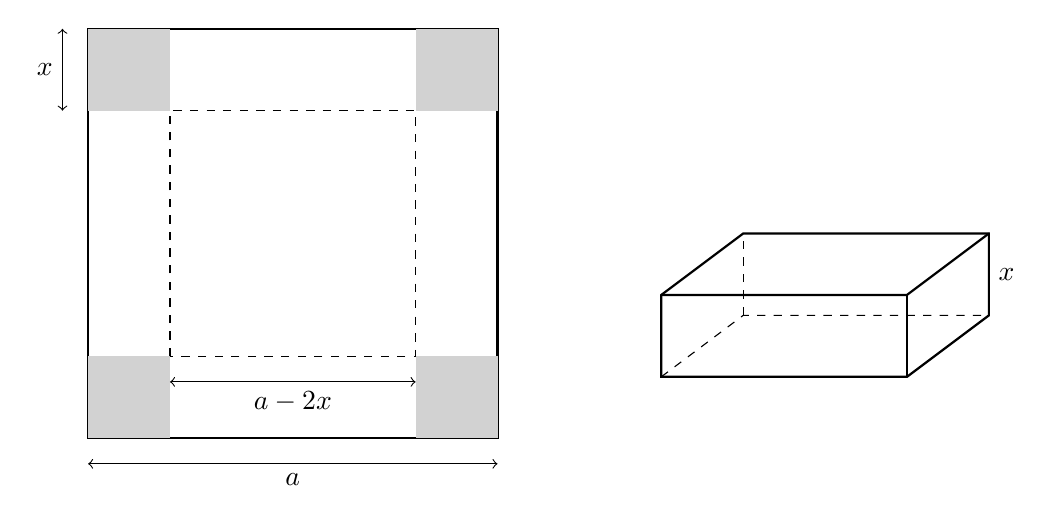
\begin{tikzpicture}[scale=1.3]
\draw[thick] (0,0) rectangle (4,4);
\foreach \p in {(0,0),(3.2,0),(0,3.2),(3.2,3.2)} {\fill[gray!35] \p rectangle ++(0.8,0.8);}
\draw[dashed] (0.8,0.8) rectangle (3.2,3.2);
\draw[<->] (0,-0.25) -- node[below] {$a$} (4,-0.25);
\draw[<->] (-0.25,3.2) -- node[left] {$x$} (-0.25,4);
\draw[<->] (0.8,0.55) -- node[below] {$a - 2x$} (3.2,0.55);
\begin{scope}[xshift=5.6cm,yshift=0.6cm]
\draw[thick] (0,0) -- (2.4,0) -- (3.2,0.6) -- (3.2,1.4) -- (0.8,1.4) -- (0,0.8) -- cycle;
\draw[thick] (0,0.8) -- (2.4,0.8) -- (3.2,1.4); \draw[thick] (2.4,0) -- (2.4,0.8);
\draw[dashed] (0,0) -- (0.8,0.6) -- (3.2,0.6); \draw[dashed] (0.8,0.6) -- (0.8,1.4);
\node[right] at (3.2,1.0) {$x$};
\end{scope}
\end{tikzpicture}
